\documentclass[12pt]{article}
\usepackage{fullpage,graphicx,psfrag,url,amsmath,amsthm,algorithm}
\usepackage{algorithmicx,algpseudocode}
\usepackage{natbib}
\usepackage{hyperref}
\usepackage[english]{babel}
\usepackage[utf8]{inputenc}
\input defs

\title{\large \bf Generalized Blind Deconvolution\\
\small Samsung Global Research Outreach Program 2017\\
\small Progress Report}
\author{Boyd Group, Stanford University}
\date{}

\bibliographystyle{alpha}

\begin{document}
\maketitle

\section{Proposal Identification}
\begin{description}
\item[Title of Proposal]\hfill\\ Generalized Blind Deconvolution
\item[Subject Theme] Machine Learning and Recognition
\item[Subject Title] Other
\item[Principal Investigator] \hfill\\
Stephen P. Boyd\\
Samsung Professor in the School of Engineering\\
Professor, Information Systems Laboratory, Department of Electrical Engineering\\
Professor (by courtesy), Department of Management Science and Engineering\\
Professor (by courtesy), Department of Computer Science\\
Institute for Computational and Mathematical Engineering\\
Stanford University\\
Packard 254, Stanford, CA 94305\\
Tel: (650) 723-0002\\
Fax: (650) 723-8473\\
\url{boyd@stanford.edu}\\
\url{http://www.stanford.edu/~boyd/}\\
\item[Co-PI Information] None.
\item[Joint Proposal] No.
\end{description}

\newpage


\section{Generalized blind deconvolution}
\emph{Blind deconvolution} is the problem of recovering a kernel and a signal from 
their (noise corrupted) convolution.
This is a ubiquitous problem in fields including signal processing, 
machine learning, communication, seismology, computer vision, microscopy, and neural science. 

We have an observation vector $y\in\reals^n$, and we seek a filter 
$w\in \reals^n$ such that the (circular) convolution $w*y\in\reals^n$ 
is close to a signal $x \in \reals^n$ that is simple under a given measure.
We formulate this as the problem
\BEQ
\begin{array}{ll}
\mbox{minimize}   & l(x-y*w)+r(x)+ s(w)\\
\mbox{subject to} &  w \in \mathcal W, \quad x \in \mathcal X
\end{array}
\EEQ
with variable $w$ and $x$.
Here $l:\reals^n \to \reals$ is a loss function that measures the approximation error,
$r:\reals^n \to \reals$ is a regularizer on the signal $x$,
$s:\reals^n \to \reals$ is a regularizer on the kernel, 
and $\mathcal W$ and $\mathcal X$ are constraint sets.
The constraint sets $\mathcal W$ and $\mathcal X$ always contain 
a \emph{normalization constraint} on $w$,
to preclude the trivial solution $w=x=0$.

We can incorporate the indicator functions of the constraints in the regularizers, 
by defining $R = r + I_{\mathcal X}$,
$S = s +I_{ \mathcal W}$. Then the problem can be expressed as
\[
\begin{array}{ll}
\mbox{minimize}   & l(x-y*w)+R(x)+ S(w),
\end{array}
\]
with variables $x$ and $w$.
The problem is convex if $l$, $r$, $s$, $\mathcal W$, and $\mathcal X$ are convex.

\paragraph{Loss.}
Common choices for the loss function are $l(u) = \|u\|_2^2$, $l(u) =\|u\|_1$. 
For the exact case, $l=I_0$, we have a equality constraint $x=y*w$.
If we have a model of the form $y=w*x+e$, where $e$ is a noise with
density $p$, we can take $l(u)=-\log p(u)$, the negative log-likelihood.

\paragraph{Signal regularizer.}
Common convex choices include
$r(x) = \|x\|_1$, total variation $\|Dx\|_1$, or Laplacian $\|Dx\|_2^2$, where $D$ is the
circular difference matrix.
Common nonconvex choices include $\|x\|_0$, the cardinality of the support of $x$, or 
$\|x\|_p^p$ with $0<p<1$.

%Another important family of choices are the higher
%other cumulants, which is to encourage the non-Gaussian property of the signal
%if we treat it as a sample of stochastic process. 

\paragraph{Kernel regularizer.} 
Common choices include the same choices as signal regularizer, such as $s(w) = \|w\|_1$, total variation $\|Dw\|_1$. 

\paragraph{Signal and kernel set.}
The signal set  $\mathcal X$ can specify simplicity, for example by limiting the cardinality
of the support of $x$.  It must also include a normalization such as 
$\|x\|=1$ for some norm $\|\cdot \|$ or $c^Tx=1$ for some nonzero $c\in \reals^n$.
The same choices can be made for $\mathcal W$.

\section{Algorithm}
We first rewrite the problem as
\[
\begin{array}{ll}
\mbox{minimize}   & l(x-z)+R(\tilde{x})+ S(\tilde{w}) \\
\mbox{subject to}  & z = y*w,\\
& w = \tilde{w},\\
& x = \tilde{x},
\end{array}
\]
with variables $w, \tilde{w}, x, \tilde{x}, z\in \reals^n$.

Then we can use the alternating direction method of multipliers (ADMM) to solve this problem,
when it is convex, or approximately solve the problem, otherwise.
% XXX GOT HERE 
The augmented Lagrangian for this problem is 
\[
\begin{array}{ll}
 \mathcal{L}_{s_1, s_2,s_3}(w, \tilde{w},x, \tilde{x}, z, u_1, u_2, u_3)=& l(x-z)+R(\tilde{x})+ S(\tilde{w})+\\
 & \frac{s_1}{2} \| z -y*w -u_1\|^2 +
 \frac{s_2}{2} \| x- \tilde{x}-u_2\|^2+
 \frac{s_3}{2} \| w- \tilde{w}-u_3\|^2,
\end{array}
\]
where $u_1, u_2, u_3$ are the scaled dual variables, and $s_1, s_2,s_3$ are positive parameters.

If we assume $l,R,S$ are all convex functions, we can define a new variable $v := (w, \tilde{w},x, \tilde{x}, z)$, 
the objective function $f(v) = f(w, \tilde{w},x, \tilde{x}, z):=l(x-z)+R(\tilde{x})+ S(\tilde{w})$, and write the linear constraints as $v\in C$. 
Then the problem is
\[
\begin{array}{ll}
\mbox{minimize}   & f(v) \\
\mbox{subject to} & v\in C,
\end{array}
\]
with variable $v$.
Then it is a convex problem with linear constraint, we can apply the standard ADMM algorithm. 
\[
\begin{array}{ll}
&v^{k+1/2} := \mathrm{prox}_{f}(v^{k}-\tilde{v}^{k})\\
&v^{k+1} :=  \Pi\left(v^{k+1/2}+\tilde{v}^k\right)\\
&\tilde{v}^{k+1} :=  \tilde{v}^k + v^{k+1/2} - v^k.
\end{array}
\]
The variable $k$ is the iteration counter, $v^{k+1/2}$ and $v^{k}$  are primal
variables, $\tilde{v}^k$ are scaled dual variables.

The proximal operator of $f$ is
\[
    \mathrm{prox}_{f}(v) = \argmin_{v'}\Big(f(v') + (\rho/2) \vnorm{v' - v}_2^2\Big),
\]
where $\rho>0$ is the proximal parameter. Here $\mathrm{prox}_{f}$ equals the sum of the proximal operators $\mathrm{prox}_{l},\mathrm{prox}_{R},\mathrm{prox}_{S}$.

The projection $\Pi$ projects the variables onto the graph of the linear constraint $C$ define by the three equations $z = y*w, w = \tilde{w}, x = \tilde{x}$. 

To compute the projection on the graph form  $z = y*w$, we can leverage the convolution theorem, 
and compute the projection of $(z,w)$ onto $z = y*w$ using its Fourier transform  $\hat z =\hat y  \circ \hat w$, where $ \circ$ is the Hadamard product.  
This update can be computed on each coordinate
\[
\begin{array}{ll}
    \hat z^{t} &= \mathcal{F}  z^{t},\\
    \hat w^{t} &= \mathcal{F}  w^{t}, \\
 (\hat z^{t+1}_i, \hat w^{t+1}_i) &= \Pi_{\hat y^{t+1}_i}(\hat z^{t+1}_i, \hat w^{t+1}_i).
\end{array}
\]
  
Here the projection is given by
\[
 \Pi_{\hat y_i}(\hat z_i, \hat w_i)= ((\hat z_i+ \hat y_i \hat w_i)/(1+\hat y_i^2), \hat y_i(\hat z_i+ \hat y_i \hat w_i)/(1+\hat y_i^2)).
\]
 Using fast Fourier transform, we can compute this update in $O(n\log n)$.
 After the coordinate-wise projection, we apply inverse Fourier transform to get 
 $z^{t+1}, w^{t+1}$.

\section{Numerical example}
 As an example, we study sparse blind deconvolution problem, where  
 $r(x) = \|x\|_1$ as a convex relaxation of the sparsity measure, $\mathcal X = \{x\in \reals^n| x_1=1\}$,
 $\mathcal W$ is the embedding of $\reals^m$ to the first $m$ coordinates of $\reals^n$, $s=0$, $l=I_{0}$ is the indicator function to impose equality.

We generate the observation $y\in \reals^n$ from the circular convolution of $w$ and $x$, namely,  $y = k*x$, 
where the signal $x\in \reals^n$ is I.I.D. sampled from the product of a Bernoulli random variable with probability $p$ and a standard Gaussian random variable,
 and the kernel $k\in \reals^n$ has an inverse $w\in \mathcal W_m \subset \reals^n$ so that $w*k = e_1$,
  where $e_1=(1,0,\ldots, 0)\in \reals^n$. 
  In the following numerical experiments, we choose the signal length $n=500$, the kernel length $m= 80$, $x$ has expected sparsity level $p=0.2$. 
  We run the above algorithm and our algorithm exactly recover the ground truth.
\begin{figure}
% 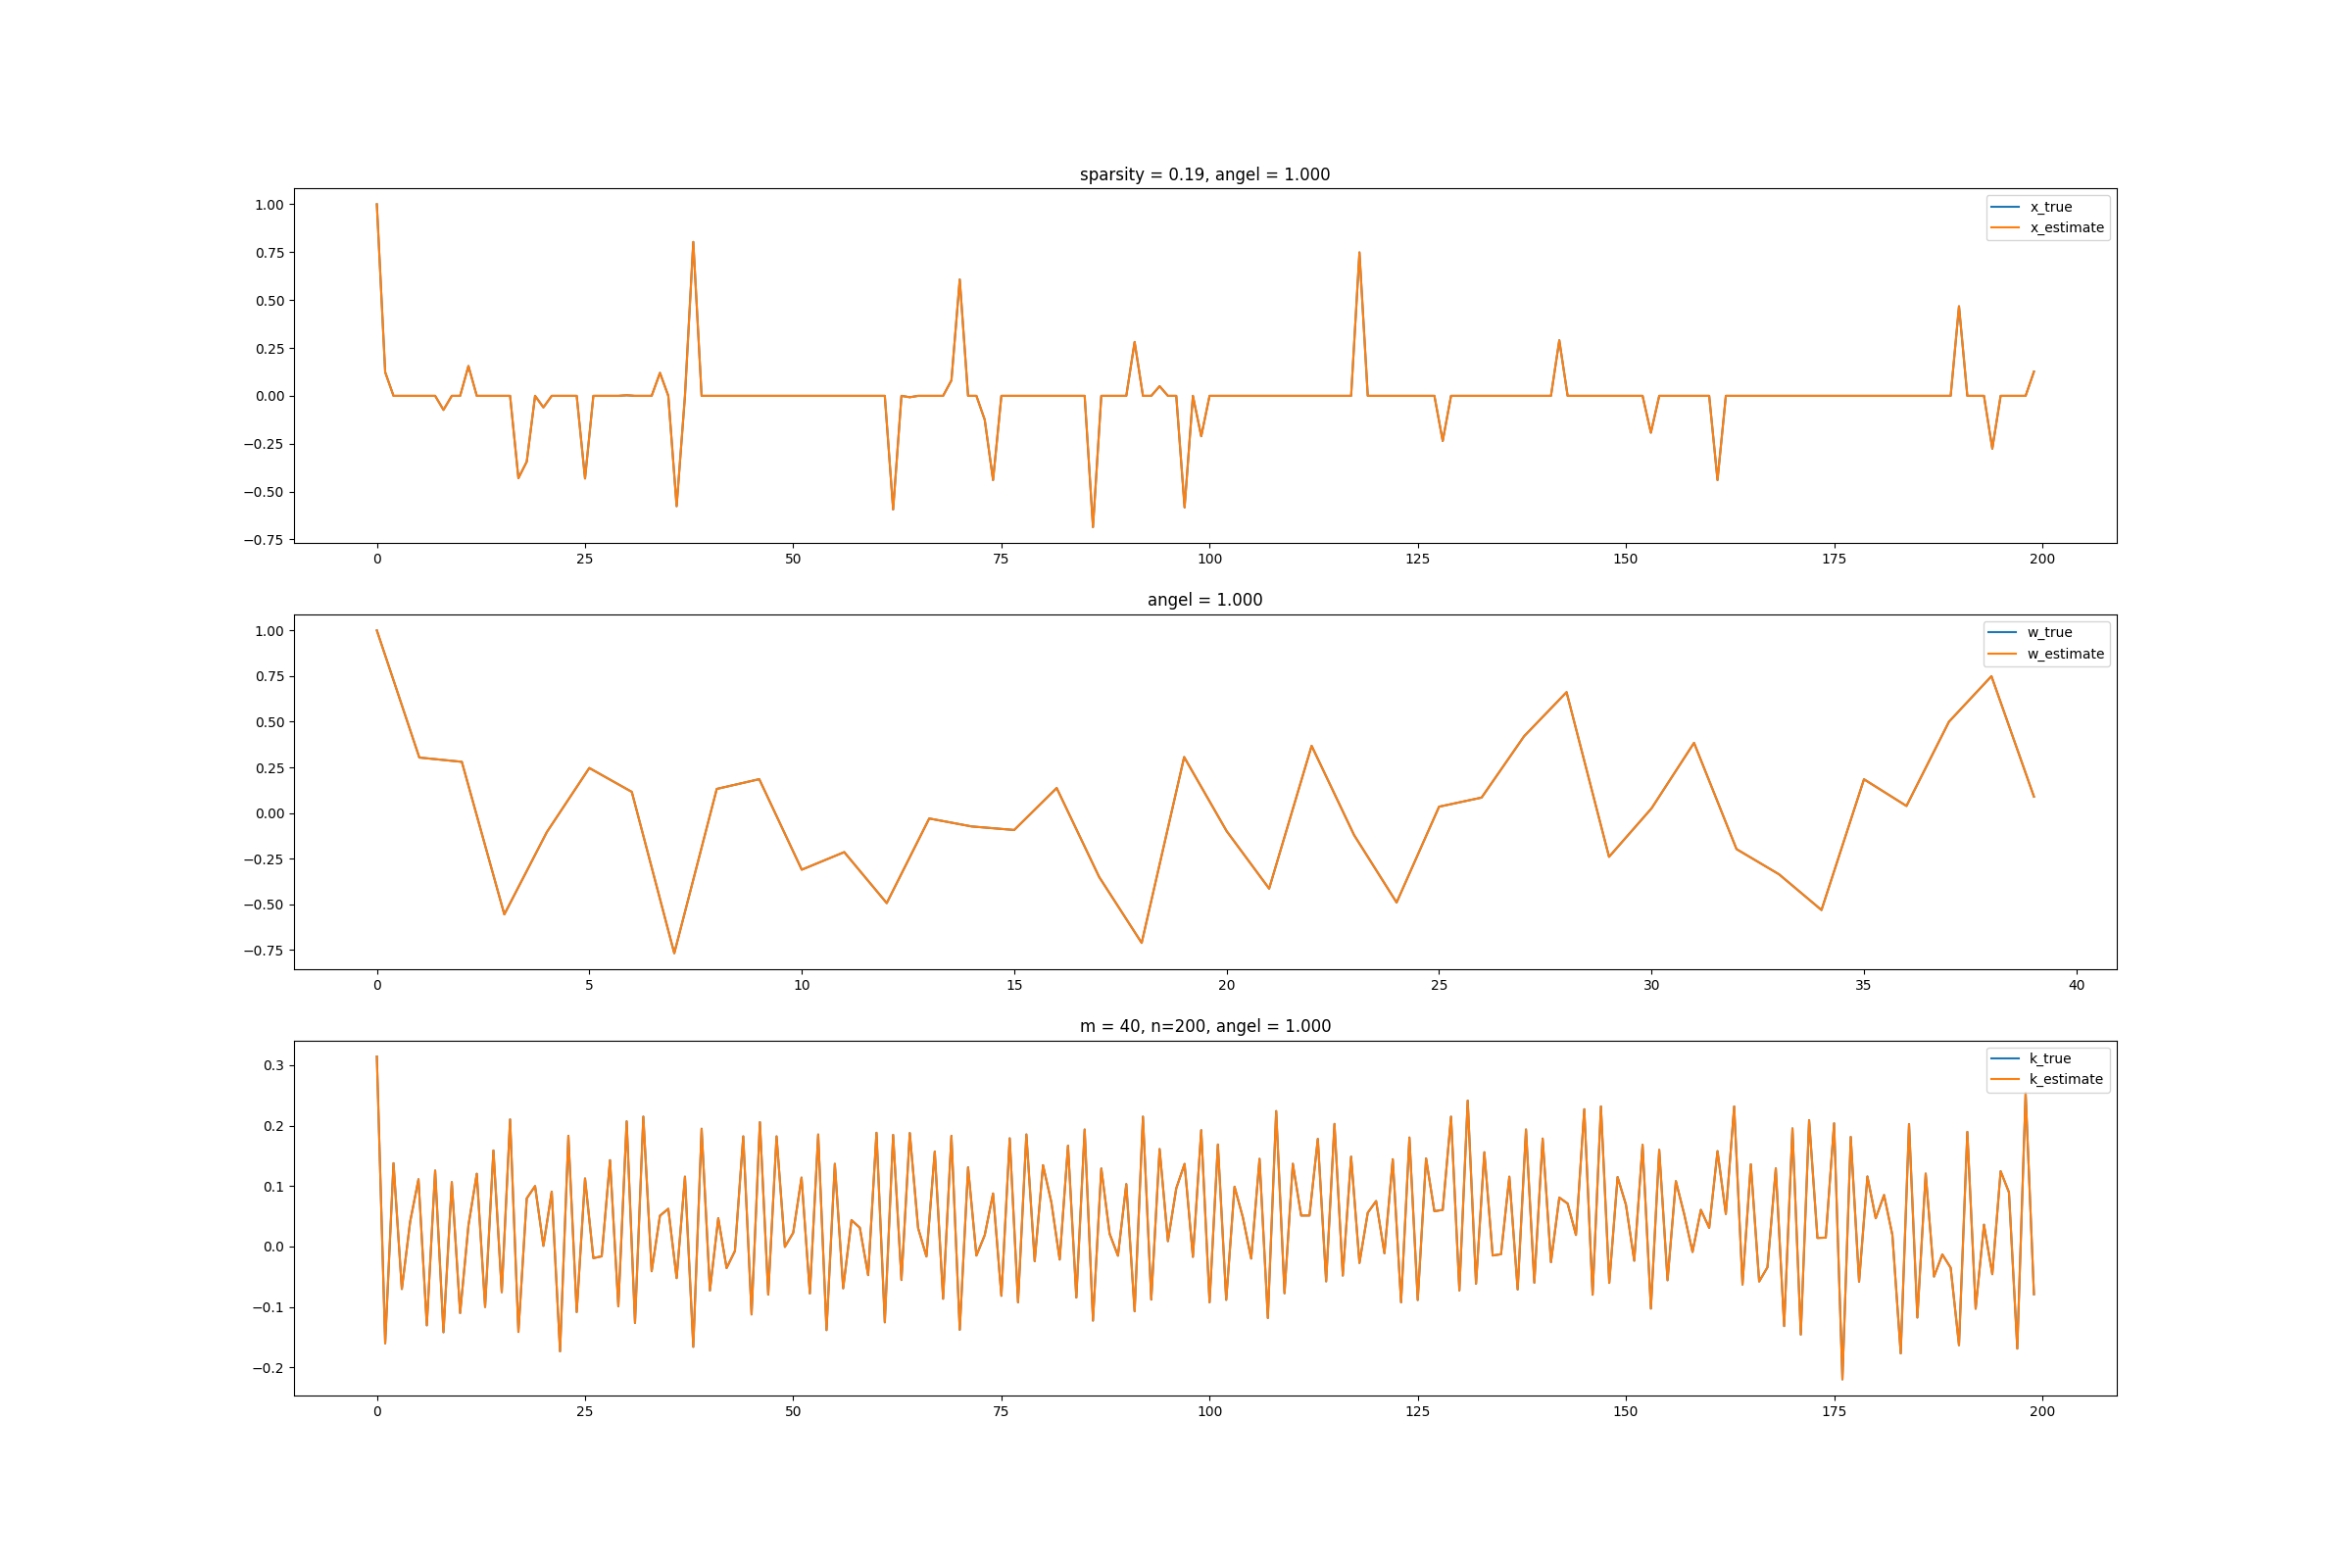
\includegraphics[width=14cm,keepaspectratio]{fig3/bShort_lenKnown_xSparse_w_Gaus_Ano_n200_k40_p0_19_sigma0_00.png}
 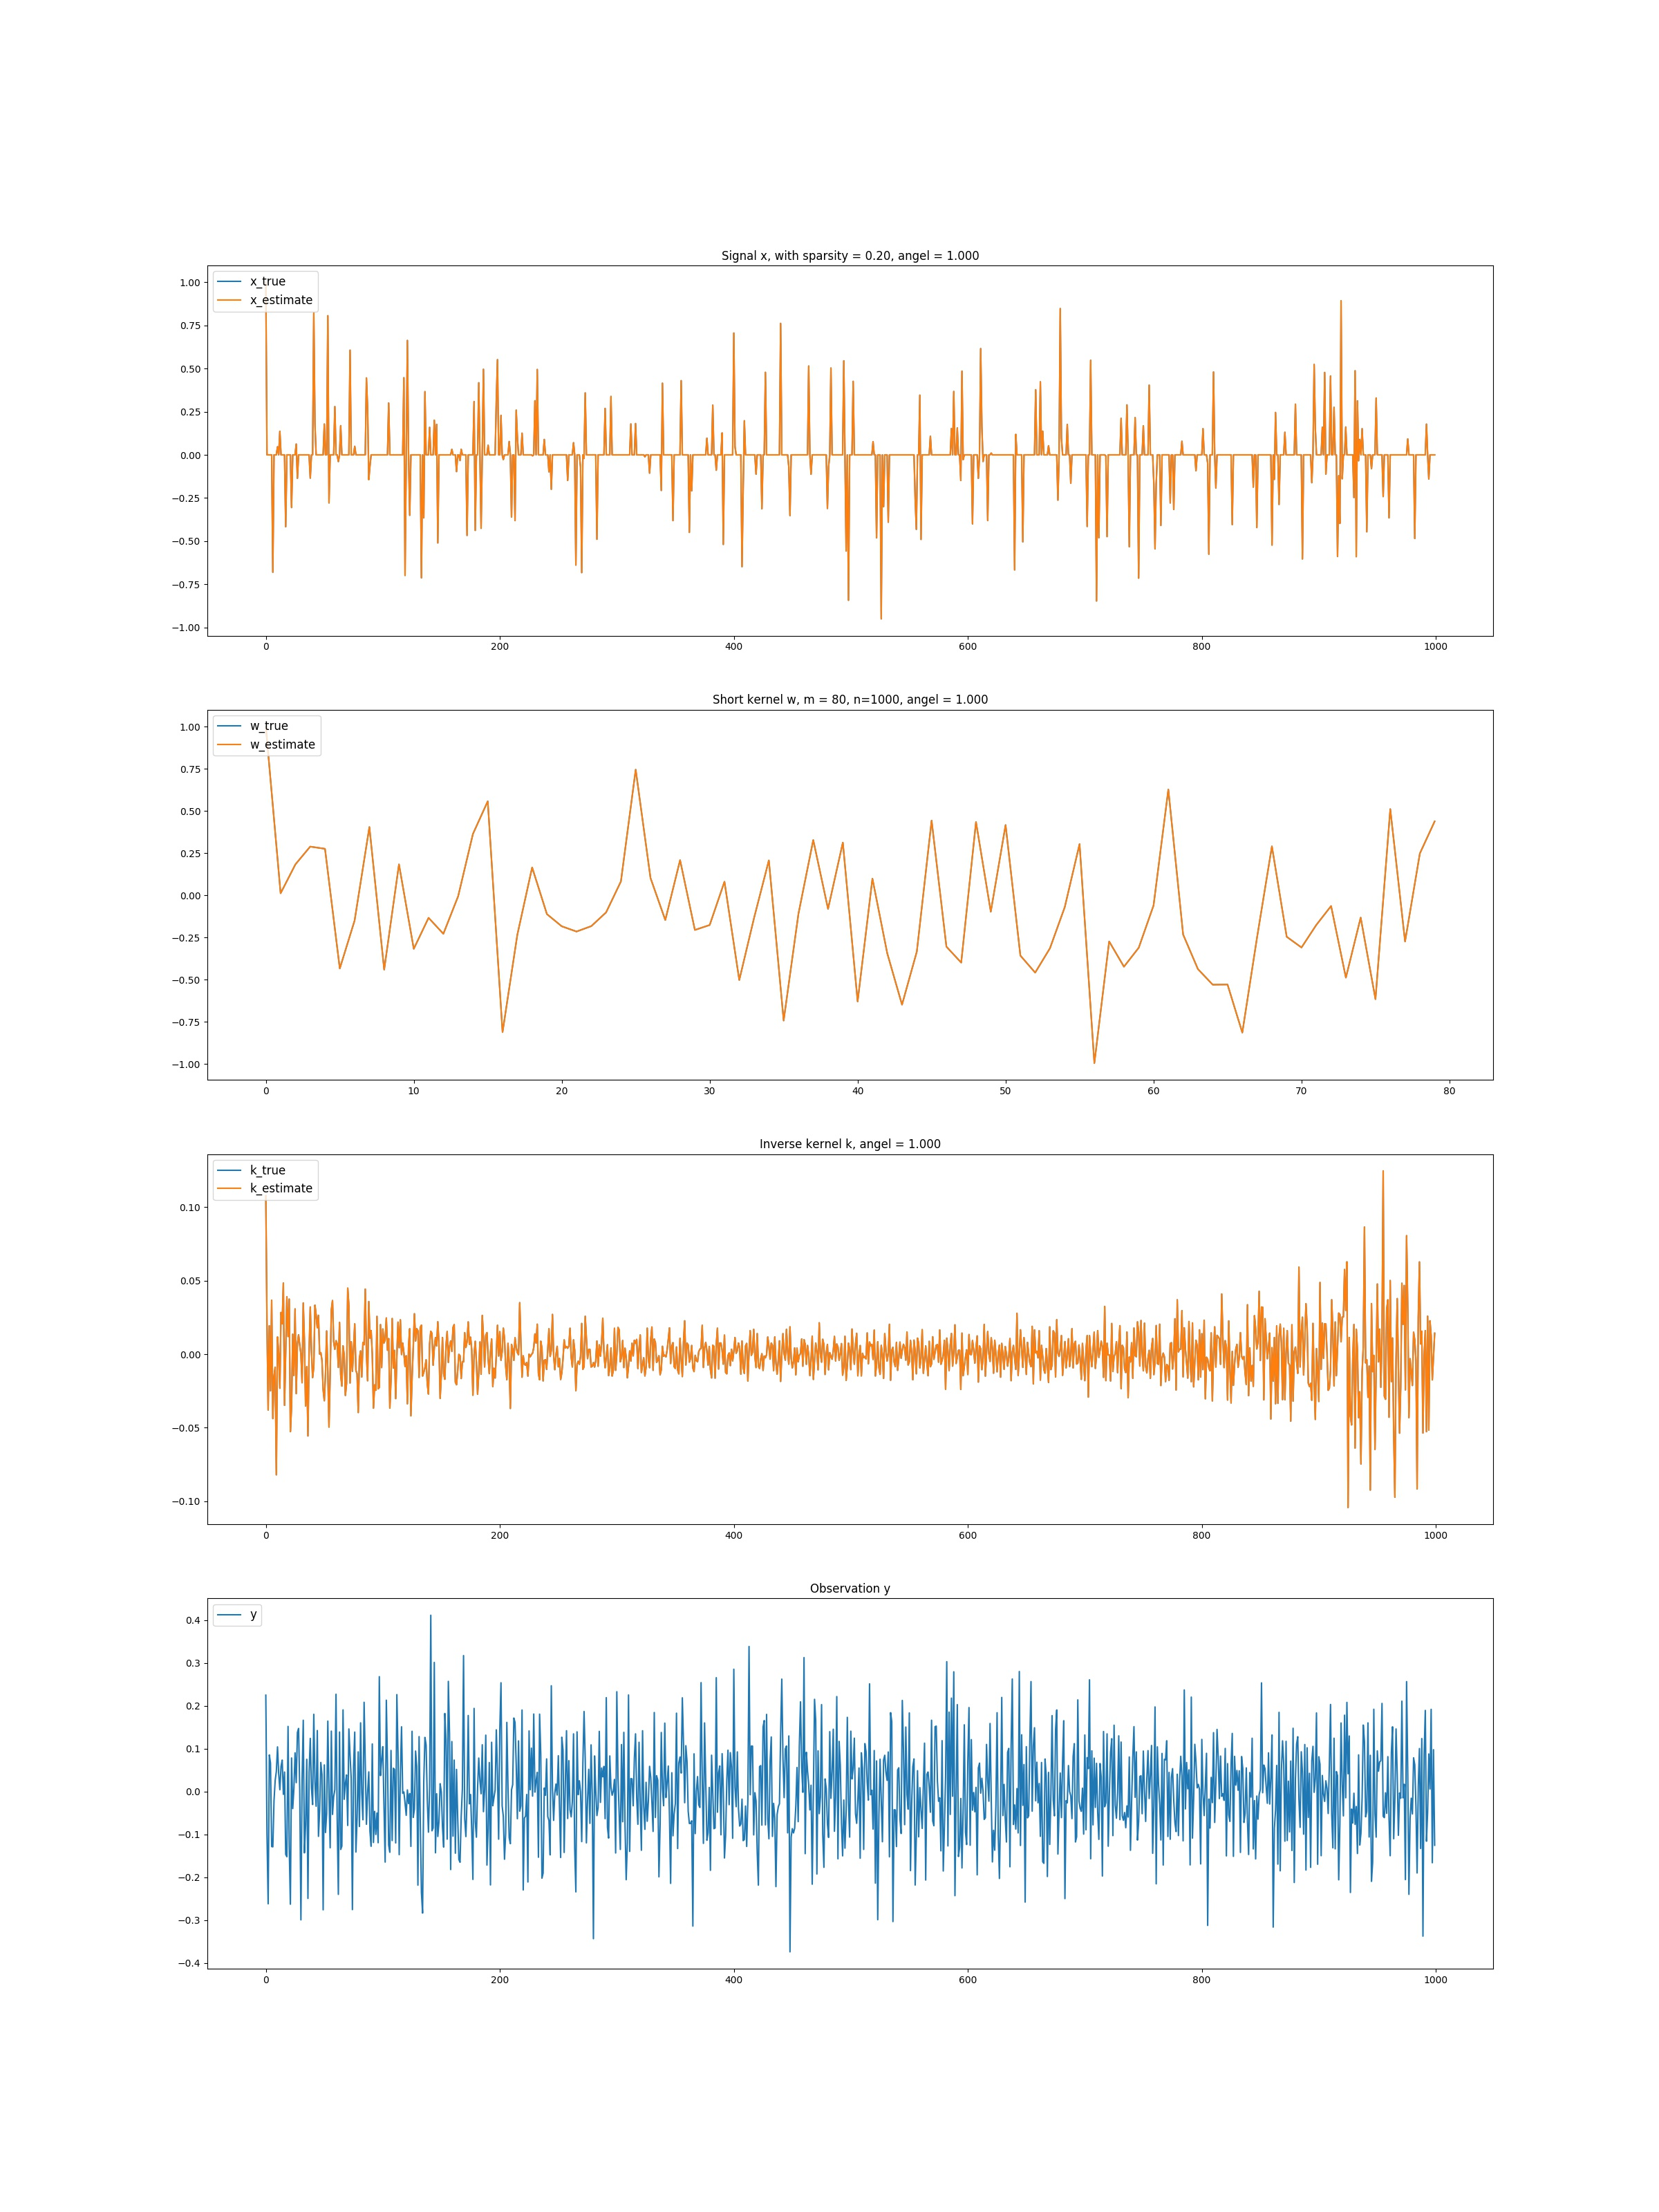
\includegraphics[width=12cm,keepaspectratio]{figures/bShort_lenKnown_xSparse_w_Gaus_Ano_n1000_k80_p0_20_sigma0_00.jpg}
\end{figure}
 
\section{Extensions and connections}
\subsection{Generative blind deconvolution }
Consider that we have an observation vector $y\in \reals^n$, and we assume that $y$ is generated by the following model,
$$y=x*k + e,$$
where $x\in \mathcal X$ is a signal and $k\in \mathcal K$ is a filter, $e$ is the error of the convolutional approximation. 
As before, the constraint sets $\mathcal X, \mathcal K$ always contain 
a \emph{normalization constraint} on $k$ because of the symmetry in $k*x$. 

Our optimization problem is
\[
\begin{array}{ll}
\mbox{minimize}   & l(y-k*x)+R(x)+ S(k)
\end{array}
\]
with variable  with variables $x,k \in \reals^n$. 
 As before, $l$ is the loss function, $R$
and $S$ are regularizers that includes the indicator function for the constraints. 

This can be viewed as synthesis approach, or generative model approach of blind deconvolution. 
The problem is non-convex, and the fundamental difficulty is that $k$ and $x$ are both unknown in $k*x$.

 We can rewrite the problem as
\[
\begin{array}{ll}
\mbox{minimize}   &  l(y-z)+R(\tilde{x})+ S(\tilde{k})  \\
\mbox{subject to}  & z = x*k,\\
& k = \tilde{k},\\
& x = \tilde{x},
\end{array}
\]
with variables $x, \tilde{x}, k, \tilde{k},z$.

Then we can use alternating direction method of multiplier (ADMM) to solve this problem. 
The augmented Lagrangian for this problem is 
\[
\begin{array}{ll}
 \mathcal{L}_{s_1, s_2,s_3}(k, x,\tilde{k},\tilde{x}, z, u_1, u_2, u_3)=&L(y,z)+R_1(\tilde{x})+ R_2(\tilde{k})
 + s_1/2 \| z -k*x -u_1\|^2 + \\
& s_2/2 \| x- \tilde{x}-u_2\|^2+s_3/2 \| k- \tilde{k}-u_3\|^2.
\end{array}
\]
Here $u_1, u_2, u_3$ are the scaled dual variables, $s_1, s_2, s_3$ are positive. 

Solving this problem is harder because $k$ and $x$ are both variable in $k*x$. 
Therefore, this problem is always non-convex. In practice, we will alternate between the updates on $k$ and $x$. 


\subsection{Connection to independent component analysis}
The generalized blind deconvolution model is closely related to Independent Component Analysis (ICA). 
In ICA, we are given an observation vector $y\in \reals^{n}$ and trying to solve the problem 
\BEQ
\begin{array}{ll}
\mbox{minimize}   &  \|Wy\|_1  \\
\mbox{subject to}  & WW^T =I
\end{array}
\EEQ
with variables $W\in \reals^{n\times n}$.

In the simplest form of sparse blind deconvolution, we are solving the problem 
\BEQ
\begin{array}{ll}
\mbox{minimize}   &  \|w*y\|_1   \\
\mbox{subject to}  & w_1=1,
\end{array}
\EEQ
with variables $w\in \mathcal{W}\subset \reals^{n}$.
 If we use the circular matrix representation of convolution, we can rewrite the problem as 
 \BEQ
\begin{array}{ll}
\mbox{minimize}   &  \|Wy\|_1   \\
\mbox{subject to}  & \frac{1}{n}\mathrm{tr}(W)=1, \\
                 &  W \mbox{ is a circulant matrix,}
\end{array}
\EEQ
with variables $W\in \reals^{n\times n}$.

 We can see that blind deconvolution is replacing the constraint that $W$ is an orthogonal matrix to that $W$ is a circular matrix with fixed trace. 
 
\subsection{Extension to deep deconvolution}
One natural extension of the discriminative blind deconvolution problem is to replace the linear convolution $w*y$ by a $m$-layer convolutional neural network. 
If we use the Relu function $\sigma(x) = \max(x, 0)$, then we can define $h_0=y$, and $h_t=\sigma(w_t*h_{t-1})$ for  $t=1,\ldots, m$.

Then the optimization problem is 
\[
\begin{array}{ll}
\mbox{minimize}& l(x-h_m)+R(x)+ S(w_1, w_2,\ldots, w_m),\\
\mbox{subject to}&h_0=y,\quad h_t=\sigma(w_t*h_{t-1}),\quad t=1,\ldots, m,
\end{array}
\]
 with the variables are $w_1,\ldots, w_m, h_1,\ldots, h_m, x$.
 
We call this problem deep deconvolution. From machine learning perspective,  blind deconvolution problem is an unsupervised learning problem. 
Our input is $y$ and output is $x$, since we don't have direct supervision on $x$, we only have a regularizer on $x$ to impose simplicity. 
This is a really hard problem, and to get a useful result from this problem, we need that the dimension of $y$ significantly longer than the size of the kernels. 

 
The generalized blind deconvolution model can be viewed an autoencoder using convolutional neural network with one hidden layer. 
Input of the neural network is $y$, and $k$ is the convolutional kernel to learn, $x$ is the hidden state, $z = k*x$ is the output of autoencoder, 
and $L(y,z)$ is the reconstruction error in this autoencoder. We can extend the model in similar fashion, then we will get a multi-layer convolutional autoencoder.



\section{Samsung contacts}

% Professor Boyd came to visit Samsung in November 2014, giving several talks.
% He has hosted several visits, including a technical visit on the GRO topic with
% Jae-Joon Han in April 2015.

%\newpage
%\section{Appendix}
%\pagenumbering{gobble}

\bibliographystyle{alpha}
\bibliography{gen_blind_deconv}

\end{document}

